\documentclass[a4paper]{article}
\usepackage{listings}
\usepackage{verbatim}
\usepackage{graphicx}
\usepackage{amsmath}
%% Language and font encodings
\usepackage[english]{babel}
\usepackage[utf8x]{inputenc}
\usepackage[T1]{fontenc}

%% Sets page size and margins
\usepackage[a4paper,top=3cm,bottom=2cm,left=3cm,right=3cm,marginparwidth=1.75cm]{geometry}

%% Useful packages
\usepackage{amsmath}
\usepackage{graphicx}
\usepackage[colorinlistoftodos]{todonotes}
\usepackage[colorlinks=true, allcolors=blue]{hyperref}

\begin{document}
\begin{titlepage}
	\raggedleft
	\rule{1pt}{\textheight} 
	\hspace{0.05\textwidth} 
	\parbox[b]{0.75\textwidth}{		
		{\LARGE\bfseries EE - 2703 Applied Programming Lab \\[0.5\baselineskip]  ~\huge Assignment -4}\\[2\baselineskip] 
		{\large\textit{Fitting Data to Models}}\\[4\baselineskip] 
		{\Large\textbf{Mohammed Khandwawala}}
        \large EE16B117
		\vspace{0.5\textheight}  
	}

\end{titlepage}


\tableofcontents


\section{Introduction}



The \textbf{Bessel functions} of the first kind J$_{n}$(x) are defined as the solutions to the Bessel differential equation.
$$x^{2}\frac{d^2{y}}{dx^{2}}+x\frac{dy}{dx}+(x^{2}-n^{2})y = 0 	$$
which are nonsingular at the origin. They are sometimes also called cylinder functions or cylindrical harmonics. This Assignment is about fitting data to models. So we will be taking two models of Bessel function and fitting them using least squares. 
The Bessel Function is given by
$$ \sqrt[2]{\frac{2}{x\pi}}cos(x-\frac{v\pi}{2}-\frac{\pi}{4}) \approx J_{v}(x)		-(1)$$ 

First Model , lets call it model(b) . Approximate value of J$_{1}$(x) can be given by,
	$$ Acos(x_{i}) + Bsin(x_{i}) \approx J_{1}(x_{i})$$
Second Model , lets call it model(c) . Its approximation is as follows.
	$$ \frac{Acos(x_{i})}{\sqrt[2]{x_{i}}} + \frac{Bsin(x_{i})}{\sqrt[2]{x_{i}}} \approx J_{1}(x_{i})$$

After fitting data to the model obtained from inbuilt Bessel function to obtain the constants . To estimate the measure of the fit we will try to get v from the constants. The closer and faster it reaches 1 the better fitting our model would be.

	From both the above fits to estimate v. From eqation (1) $$\phi = \frac{v\pi}{2}+\frac{\pi}{4}$$
    and $$cos(\phi) = \frac{A}{\sqrt[2]{A^{2}+B^{2}}}$$
So, 
$$ v = \frac{2}{\pi}(cos^{-1}(\frac{A}{\sqrt[2]{A^{2}+B^{2}}}))-\frac{\pi}{4})$$

\section{About Least Squares Fitting}

Solves the equation A X = B by computing a vector x that minimizes the Euclidean 2-norm $\parallel\parallel b - a x \parallel\parallel$ $^{2}$. The equation may be under\-, well\-, or over- determined (i.e., the number of linearly independent rows of a can be less than, equal to, or greater than its number of linearly independent columns). If a is square and of full rank, then X (but for round-off error) is the “exact” solution of the equation.
From linear algebra package of numpy lstsq function does the work for us which is used in the assignment to solve matrix equations by least square.

\subsection{Function Definition}

Defining function to return the value of Bessel function of v=1.For this we are using inbuilt function from python. It is included under special functions in scipy package.  

\begin{lstlisting}[language=Python ,caption=Defining Functions]
from scipy import linalg,special
#defining approximate bessel function
def J(x,v): 	
	return special.jv(1,x)

\end{lstlisting}

As mentioned in the problem statement , a vector of 40 length from 0-20 with 40 step size is created and it is passed to bessel function. The functional values obtained are plotted against the vector. NOTE : Bessel funtion was not defined at 0 and thus only plotted from 0.5.See figure 1.

\begin{lstlisting}[language=Python ,caption=Plotting the functions]
x = np.linspace(0.5,20,40)

#calculating bessel function for v = 1
jx1 =  J(x,1)

#plotting J1x
plt.plot(x,jx1)
plt.ylabel("J$_{v}$(x)")
plt.xlabel("x")
plt.grid(True)
plt.title("x vs bessel function for v=1")
plt.show()
\end{lstlisting}
\begin{figure}
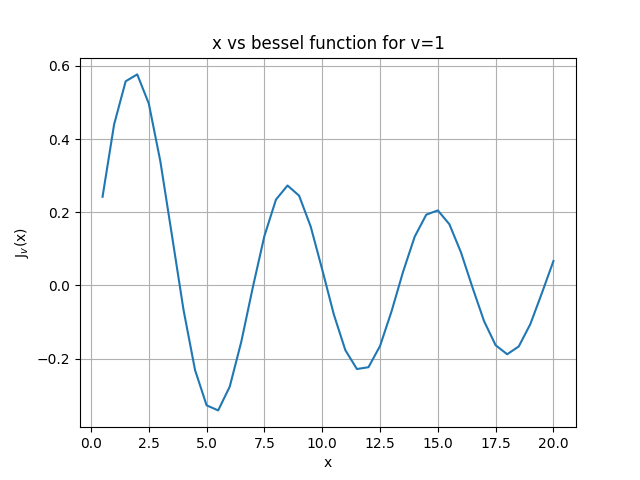
\includegraphics[width=\columnwidth]{Figure_1.png}
\caption{Plot of bessel function with v=1}
\end{figure}

\subsection{Estimation of  v}
In earlier section model(b) and model(c) and the way to estimate v are already defined and the way to estimate v. Model(b) can be converted to the matrix equation given.
\begin{gather}
 \begin{bmatrix} cos(x) & sin(x) \\  cos(x+h) & sin(x+h)  \\ ... & ... \\cos(x_{o}) & sin(x_{o}) \end{bmatrix}
 \begin{bmatrix}
 A\\ B 
 \end{bmatrix}
 =
  \begin{bmatrix}
 J_{1}(x) \\ J_{1}(x+h) \\ ... \\ J_{1}(x_{o})
   \end{bmatrix}
\end{gather}
Following naming convention for the corresponding matrix is used in the code.
$$ M1 M2 = M3 $$

Here h is step size. Solving this equation multiple times for 0 < x < x$_{o}$ using least square. For each solution v is calculated and plotted. 
\subsubsection{Estimation of v for model(b)}
For x$_{o}$ different A,B values are obtained and the v is calculated by comparing cos$_{-1}\phi$ with phase. And then then the obtained values of v are plotted against x.See Figure 2.
\begin{lstlisting}
v=[]
#To store v from second method
v_2=[]
for i in range(0,37):
	x1 = x[i:40]
	#to get matrix with sinusoids 
	M1_1 = np.transpose(sincos(x1))
	#to get A,B using least square by matrix approach	
	M3_1 = J(x1,1)
	coeff = linalg.lstsq(M1_1,M3_1)[0]
	phi = coeff[0]/np.sqrt(coeff[0]**2+coeff[1]**2)
	v.append((2/np.pi)*(np.arccos(phi)-np.pi/4))

\end{lstlisting}

\subsubsection{Estimation of v for model(c)}
Similar to model (b) just the M1 matrix will change Now,
\begin{gather}
M1 = 
\begin{bmatrix} \frac{cos(x)}{\sqrt[2]{x}} & \frac{sin(x_{o})}{\sqrt[2]{x}} \\  \frac{cos(x+h)}{\sqrt[2]{x+h}} & \frac{sin(x+h)}{\sqrt[2]{x_{o}+h}}  \\ ... & ... \\\frac{cos(x_{o})}{\sqrt[2]{x_{o}}} & \frac{sin(x_{o})}{\sqrt[2]{x_{o}}} \end{bmatrix}
\end{gather}
 For x$_{o}$ different A,B values are obtained and the v is calculated by comparing cos$_{-1}\phi$ with phase. And then then the obtained values of v are plotted against x. See Figure 2.
\pagebreak
\begin{lstlisting}

for i in range(0,37):
	x1 = x[i:40]
	#creating matrix with sinusoids by root x 
	M1_2 = np.transpose(sincos2(x1))
	print M1_2
	#to get A,B using least square by matrix approach
	M3_2 = J(x1,1)
	print M3_2
	coeff2 = linalg.lstsq(M1_2,M3_2)[0]
	phi_2 = coeff2[0]/np.sqrt(coeff2[0]**2+coeff2[1]**2)
	print phi_2
	v_2.append((2/np.pi)*(np.arccos(phi_2)-np.pi/4))

\end{lstlisting}

\begin{lstlisting}
plt.plot(v,"go")
plt.plot(v_2,"bo")
plt.title("Value of v computed")
plt.legend(["model (a)","model (b)"])
plt.show()

\end{lstlisting}
\begin{figure}
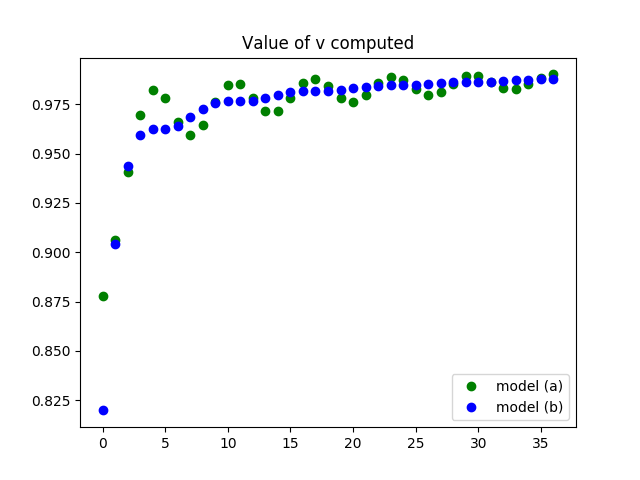
\includegraphics[width=\columnwidth]{Figure_1-1.png}
\caption{plotting value of v obtained by both the models}
\end{figure}
\subsubsection{Figure 2 observation}
As it can easily be seen from figure 2 that model (c) converges faster . And hence model(b) is more accurate than model (b). Convergence in both the models is less than but close to 1.
\subsection{Defining function to calculate v}
The Defined function is of the for as required in the problem statement
$$calcnu(x,x0,color,eps,model)$$
\begin{itemize}
\item x : input vector from 0 to 20 (any step size)
\item xo : limit of x
\item color : Color for plotting
\item eps : noise value
\item model : model(b) or (c)
\end{itemize}

Noise : We will add some noise to M3 matrix that is the matrix of functional value. Noise is added using python random.randn which returns sample form standard normal distribution. 
\begin{lstlisting}
def calcnu(x,xo,color,eps,model):
	if model == "b" :
		v=[]
		for i in range(0,(len(x)/20)*xo+1):
			x1 = x[i:len(x)]
			print i	
			M1_1 = np.transpose(sincos(x1))
			M3_1 = J(x1,1)
			coeff = linalg.lstsq(M1_1,M3_1+eps*np.random.randn(len(x1)))[0] 
			#adding noise to the functional values
			phi = coeff[0]/np.sqrt(coeff[0]**2+coeff[1]**2)
			#computing phase and than obtaining v
			v.append(((2/np.pi)*(np.arccos(phi)-np.pi/4)))
	if model == "c" :
		v=[]
		for i in range(0,(len(x)/20)*xo+1):
			x1 = x[i:len(x)]
			M1_2 = np.transpose(sincos2(x1))
			M3_2 = J(x1,1)
			coeff2 = linalg.lstsq(M1_2,M3_2+eps*np.random.randn(len(x1)))[0] 
			#adding noise to the functional values
			phi_2 = coeff2[0]/np.sqrt(coeff2[0]**2+coeff2[1]**2)
			#computing phase and than obtaining v
			v.append((2/np.pi)*(np.arccos(phi_2)-np.pi/4))
	plt.plot(x[0:(len(x)/20)*xo+1],v,color)

\end{lstlisting}

\subsection{Plotting using calcnu function}

Plotting three different plots. First plot is of model (b) with no noise , second plot of model (c) with no noise and third model with noise of O.O1 on model(c). See Figure 3.

\begin{lstlisting}
	
calcnu(x,18,"go",0,"b")
calcnu(x,18,"bo",0,"c")
calcnu(x,18,"ro",0.01,"c")
plt.grid(True)
plt.legend(["e = 0, model (b)","e = 0, model (c)","e = 1.0e-02, model (c)"])
plt.show()

\end{lstlisting}
\begin{figure}
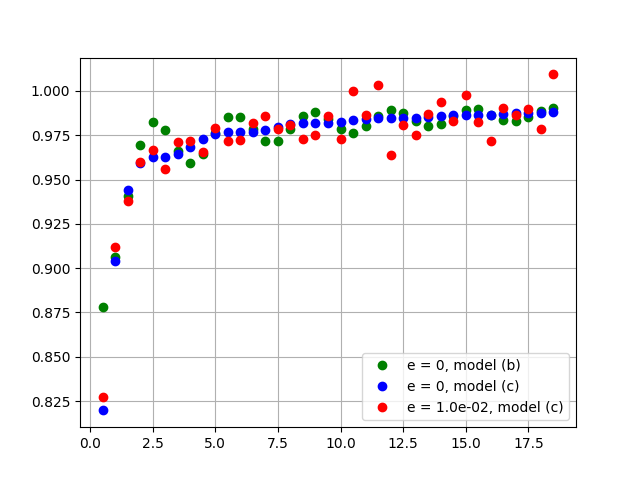
\includegraphics[width=\columnwidth]{Figure_1-2.png}
\caption{Plotting for v using model (b) with and without noise ans (c)}
\end{figure}
\subsubsection{Observation from Figure 3}
It can be seen that model(c) with noise has more variance . But mean still seems to be centered around the old convergence value. Adding noise increases error in out estimation of v for large value of x$_{o}$ which earlier was more accurate.
\subsection{Effect on Varying measurements}
The effect of number of measurements is not observed for no noise.In case of noise (See Figure 4 for model(b) and Figure 5 for model(c)) When the the number of measurements are increased and the same amount if noise is added , since our calculation has value of bessel function at more number of point effect of noise is reduced. Clearly from the plot the red triangles are more distorted with are calculated taking 40 points then blue crosses which were evaluated taking 1000 points.This result is consistent in both the models because it does not depend on the model but is a general property.
\begin{lstlisting}

x_2 = np.linspace(0.5,20,40)
x_3 = np.linspace(0.5,20,1000)


calcnu(x_2,18,"r^",0.005,"b")
calcnu(x_3,18,"b+",0.005,"b")

plt.title("Variation in (b) model with number of measurements with noise")
plt.grid(True)
plt.legend(["with 40 measurements","with 1000 measurements"])
plt.show()

\end{lstlisting}
\begin{figure}
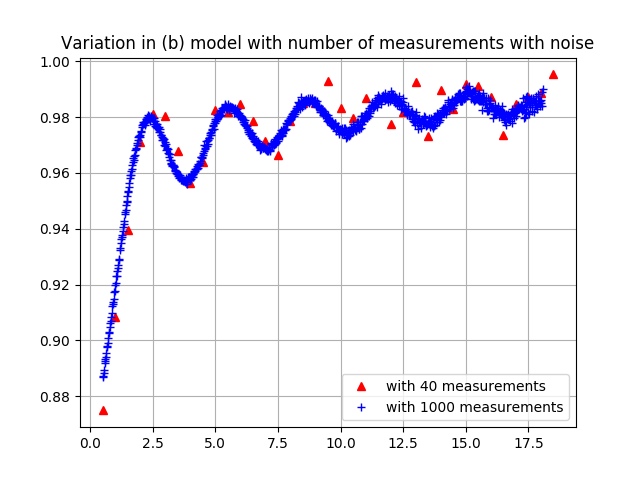
\includegraphics[width=\columnwidth]{Figure_1-3b.png}
\caption{Variation in (b) model with number of measurements with noise}
\end{figure}

\begin{lstlisting}
calcnu(x_2,18,"r^",0.005,"c")
calcnu(x_3,18,"b+",0.005,"c")

plt.title("Variation in (c) model with number of measurements with noise")
plt.grid(True)
plt.legend(["with 40 measurements","with 1000 measurements"])
plt.show()
\end{lstlisting}
\begin{figure}
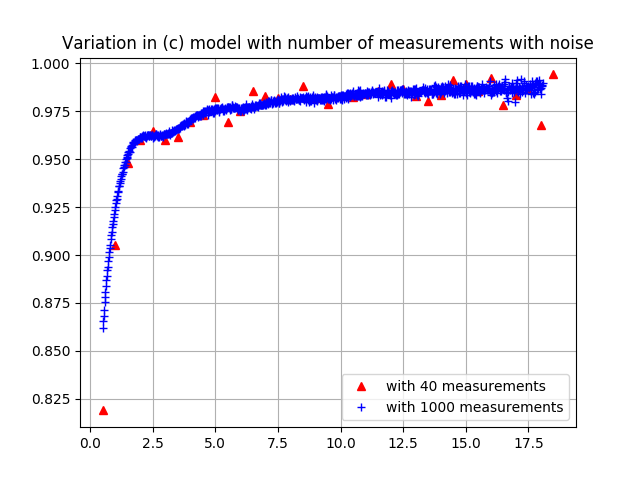
\includegraphics[width=\columnwidth]{Figure_1-4b.png}
\caption{Variation in (c) model with number of measurements with noise}
\end{figure}
\subsection{Effect of varying noise}
Plotting both the models with different amount of noise 0 , 0.001, 0.003 and 0.005. Similar results are obtained in both the models. For Higher x$_{o}$ values estimated v starts blowing up even for low noise content. For 0.01 nature of the curve is distinguishable and for 0.05 noise dominates. Quality of the fit reduces as the level of noise increases.  See Figure 6 and Figure 7.

\begin{lstlisting}
calcnu(x,18,"go",0,"b")
calcnu(x,18,"b^",0.05,"b")
calcnu(x,18,"c+",0.03,"b")
calcnu(x,18,"rx",0.01,"b")
plt.grid(True)
plt.title("Variation in (b) model with noice")
plt.legend(["e = 0, model (b)","e = 0.05, model (b)","e = 0.03, model (b)","e = 0.01, model (b)"])
plt.show()

\end{lstlisting}
\begin{figure}
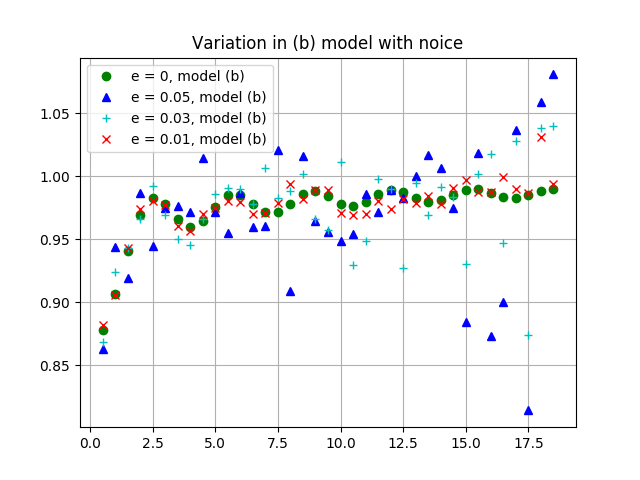
\includegraphics[width=\columnwidth]{Figure_1-5.png}
\caption{Variation in (B) model with noise}
\end{figure}

\begin{lstlisting}
calcnu(x,18,"go",0,"c")
calcnu(x,18,"b^",0.05,"c")
calcnu(x,18,"c+",0.03,"c")
calcnu(x,18,"rx",0.01,"c")
plt.grid(True)
plt.title("Variation in (c) model with noise")
plt.legend(["e = 0, model (c)","e = 0.05, model (c)","e = 0.03, model (c)","e = 0.01, model (c)"])
plt.show()
\end{lstlisting}

\begin{figure}
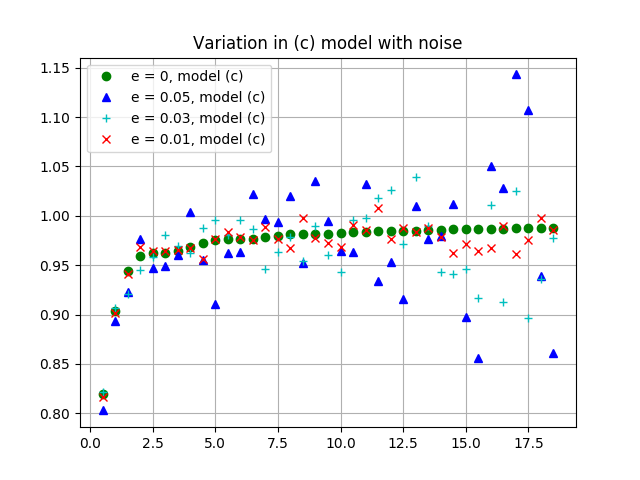
\includegraphics[width=\columnwidth]{Figure_1-6.png}
\caption{Variation in (C) model with noise}
\end{figure}
\subsection{Quality of the Fit}
To have good quality of fit from a model Increase in step-size can compensate for noise. Figure - 8 and Figure - 9 show model (b) and model (c) with varying noise just like Figure -6 and Figure -7. Significantly better result is obtained even for higher noise values .  
\begin{lstlisting}
calcnu(x_3,18,"go",0,"b")
calcnu(x_3,18,"b^",0.05,"b")
calcnu(x_3,18,"c+",0.03,"b")
calcnu(x_3,18,"rx",0.01,"b")
plt.grid(True)
plt.title("Variation in (b) model with noise 1000 points")
plt.legend(["e = 0, model (b)","e = 0.05, model (b)","e = 0.03, model (b)","e = 0.01, model (b)"])
plt.show()
\end{lstlisting}

\begin{figure}
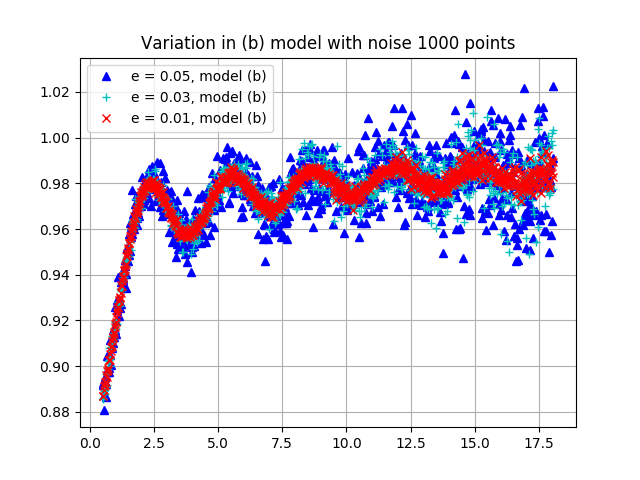
\includegraphics[width=\columnwidth]{Figure_1-7.png}
\caption{Variation in (b) model with noise and step-size}
\end{figure}

\begin{lstlisting}
calcnu(x_3,18,"go",0,"c")
calcnu(x_3,18,"b^",0.05,"c")
calcnu(x_3,18,"c+",0.03,"c")
calcnu(x_3,18,"rx",0.01,"c")
plt.grid(True)
plt.title("Variation in (c) model with noise 1000 points")
plt.legend(["e = 0, model (c)","e = 0.05, model (c)","e = 0.03, model (c)","e = 0.01, model (c)"])
plt.show()
\end{lstlisting}

\begin{figure}
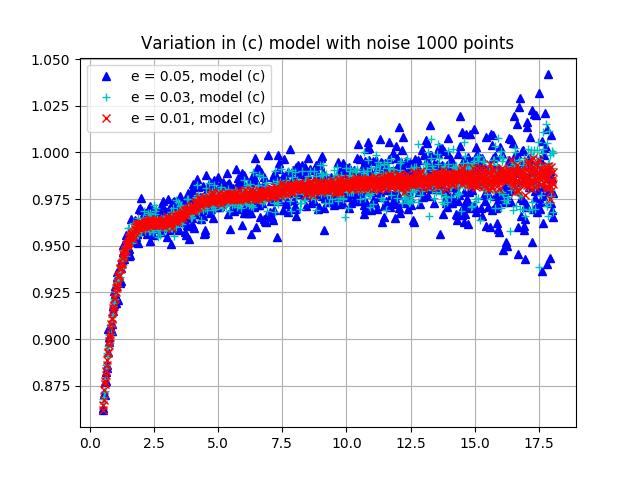
\includegraphics[width=\columnwidth]{Figure_1-8.png}
\caption{Variation in (C) model with noise and step-size}
\end{figure}

\end{document}